\documentclass[10pt]{article}
\usepackage[a4paper, total={7in,10in}]{geometry}
\usepackage{hyperref}
\usepackage{siunitx}
\usepackage{graphicx}
\usepackage{caption}
\usepackage[backend=biber]{biblatex}
\addbibresource{report.bib}

%opening
\title{EP2420 Project 2 - Forecasting Service Metrics}
\author{André Silva}
\begin{document}

\maketitle

\section*{Task III}
\label{sec:3}

In this task we apply traditional univariate forecasting methods, namely the autoregression (AR) and the moving average (MA) models.

AR is a model that provides a linear mapping from past observations to the next step of a time series, while MA defines the output as a linear function of past residual error values.

As we will be studying the impact of each of these models given their parameters, as well as the horizon of the predictions, it is useful to also look at a well known method for model identification. 

The autocorrelation is a measurement of the correlation between one value and its predecessors. It is a useful tool for better understanding time series, from where we can extract, for example, information about seasonality and trend. Figures \ref{fig:3} and \ref{fig:4} show us, respectively, the ACF and the PACF, where we can see the respective values for each \textit{lag}, as well as the $95\%$ confidence intervals represented by the light blue funnels.

\begin{figure}[!ht]
    \centering
    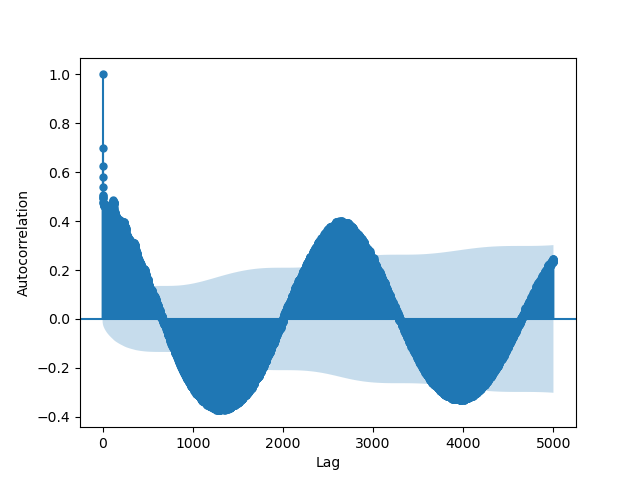
\includegraphics[width=0.40\textwidth,height=\textheight,keepaspectratio]{../acf.png}
    \caption{Plot of the autocorrelation function (ACF) of our time series}
    \label{fig:3}
\end{figure}

\begin{figure}[!ht]
    \centering
    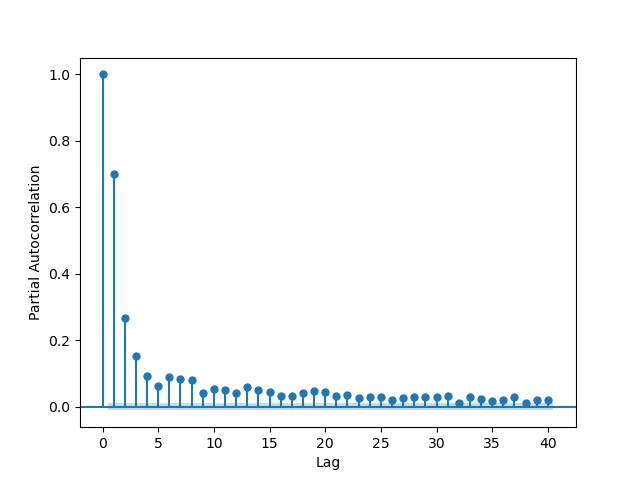
\includegraphics[width=0.40\textwidth,height=\textheight,keepaspectratio]{../pacf.png}
    \caption{Plot of the partial autocorrelation function (PACF) of our time series}
    \label{fig:4}
\end{figure}

Figure \ref{fig:3} shows a clear seasonality in our time series, which can be explained by the way our data was generated in ~\cite{9012741}, following a Poisson process in which the arrival rate is modulated by sinusoidal function.

\pagebreak

To perform our experiment, we split the trace into training and test sets ($70/30$). Since we will be studying univariate methods, we only need the target variable, \textit{ReadsAvg}.

After this, we transform the test set into a list of pairs that follow the structure $([x^{(t-l)},...,x^{(t-1)}],[y^{(t)},...,y^{(t+h)}])$, in which $l$ is either $p$ or $q$, dependent on which model we are studying. As we are using analyzing \textit{KV periodic}~\cite{9012741}, our step size (i.e. time between each sample of a sequence), is $1$ second. By using this transformed dataset in our experiments, we are able to conclude on the impact of the parameters $p$ and $q$, as well as compare them with the results from previous tasks.

We then perform an experiment to study the impact of $p$ and $q$ on the accuracy of our models and its predictions of $0...10$ steps into the future by building $10$ different models with $p,q\in\{1,...,10\}$ and performing rolling forecast for each pair of the test set.

Figures \ref{fig:5} and \ref{fig:6} show us the \textsc{NMAE} of each model when predicting $y^{(t+h)}$. Rows represent the time horizon $h = 0,...,10$ and columns represent the lag $p,q = 1,...,10$. The color gradient of the heat-map allows us to visualize and extract conclusions better than if we used a normal table.

\begin{figure}[h!]
    \centering
    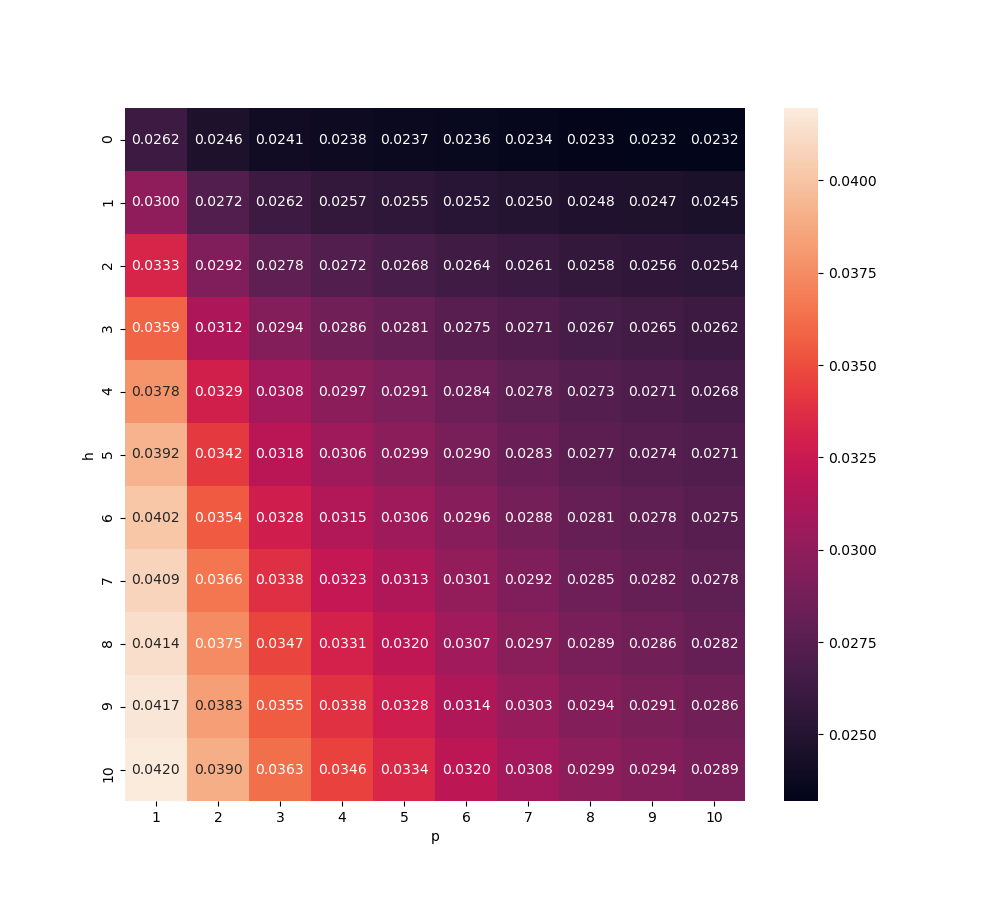
\includegraphics[width=0.65\textwidth,height=\textheight,keepaspectratio]{../ar_nmae_heatmap.png}
    \caption{Heat-map of \textsc{NMAE} for each AR model with $p\in\{1,...,10\}$ when predicting $y^{(t+h)}$}
    \label{fig:5}
\end{figure}

When we analyze the results of Figure \ref{fig:5} by looking at each row, we notice that there is a clear trend in all of them, where the \textsc{NMAE} decreases as we increase $p$. On the other hand, when we look at each column, we see that the \textsc{NMAE} increases as we increase $h$. Both of these events are, intuitively, expected. When we increase $p$, we are utilizing more information, or context, for each prediction, so we expect better predictions. This can also be explained by \ref{fig:3}, where we clearly see that previous results in the considered range of lag have influence in the current state. When we increase $h$, we are asking for a value that is more distant in time, for which the models have to make more assumptions, and so, have a worse accuracy.

We should also note that, even though this model is suitable for series without trend and seasonal components and our series has both, as shown in Figure \ref{fig:3}, it is still able to obtain good results.

\pagebreak

\begin{figure}[h!]
    \centering
    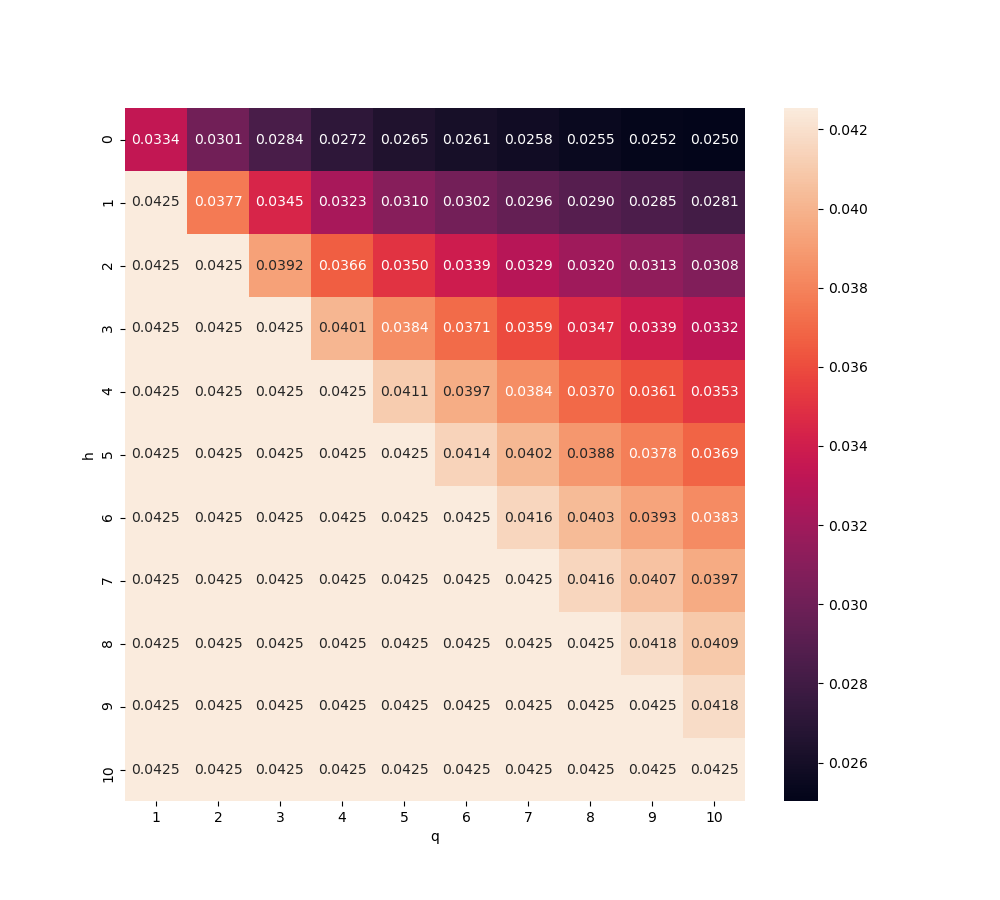
\includegraphics[width=0.65\textwidth,height=\textheight,keepaspectratio]{../ma_nmae_heatmap.png}
    \caption{Heat-map of \textsc{NMAE} for each MA model with $q\in\{1,...,10\}$ when predicting $y^{(t+h)}$}
    \label{fig:6}
\end{figure}

The most noticeable aspect of Figure \ref{fig:6} are the values below the diagonal, where all the results have the same value. This is explained by the definition of the MA model, in which the next value is a linear function of past residual errors. The values below the diagonal represent predictions where $h \geq q$, so all the residual errors utilized are $0$, as this is the value considered during our rolling forecast, and so the predictions are all equal to the constant values, which in is case is equal for every model as it is the mean of the training set.

When we analyze the results by looking at each column, we notice that the \textsc{NMAE} increases as we increase $h$, even on the upper part of our heat-map. This is, again, explained by our rolling forecast method, which, converted to common language, means that we are trying to predict further into the future and, to do so, making more assumptions about the process. 

When we analyze by looking at each row, we are not able to extract any conclusion from these. The only explanation we could identify for this is the fact that we are utilizing a method suitable for series without trend and seasonal components, which is not the case of our series, as shown in Figure \ref{fig:3}.

If we compare the AR and MA models, we can see that the AR model clearly outperforms the MA model. When compared to the previously studied models, we see that the AR model is the best model when predicting the current state (i.e. $h=0$), while it is outperformed by the LSTM model for $h>0$, and even by the Linear Regressor for larger values of $h$. On the other hand, the MA model isn't able to outperform any of them, being the worst performing model so far.

\printbibliography

\end{document}
